\section{Intelligence Artificielle}

\subsection{Stratégies}
\subsubsection{Intelligence aléatoire}
Lorsque le personnage est dans une salle de combat, il joue aléatoirement des cartes jusqu'à une éventuelle fin de combat. Il peut aussi choisir de finir son tour. Lorsqu'il est dans la salle de repos, il choisira aléatoirement entre se soigner ou améliorer ses statistiques. Lorsqu'il est dans une salle d'entrainement ou si le joueur à remporté un combat, le personnage choisira aléatoirement une carte parmis les trois proposées pour rajouter à son deck, ou choisira de passer à la salle suivante directement. Si il est à l'exterieur d'une salle, et donc sur la carte, la seule option disponible est de rentrer dans la salle suivante.
\clearpage

\subsection{Conception logiciel}
Le diagramme des classes pour l’intelligence artificielle est présenté en \autoref{uml:ai}.

\underline{\textbf{AI\_Random}}
\par Classe implantant l'intelligence aléatoire.

\clearpage

\begin{figure}[hp]
\includegraphics[width=0.6\paperheight]{images/ai.png}
\caption{\label{uml:ai}Diagramme des classes d'intelligence artificielle.} 
\end{figure}

\clearpage
%\begin{landscape}
%\begin{figure}[p]
%\includegraphics[width=0.9\paperheight]{ai.pdf}
%\caption{\label{uml:ai}Diagramme des classes d'intelligence artificielle.} 
%\end{figure}
%\end{landscape}
